The team worked together as described in the  two following sub-sections: i) Project organisation (structure of the team, where functionality and administrative task were assigned) and ii) Decision making and conflict resolution methodologies (i.e. How we make decisions and solve conflicts or disagreements as a team).

\subsection{Project Organisation}

5.1.1  Roles

All team members have two type of tasks: i) core tasks (e.g. programming goals) and ii) administrative tasks (e.g. documentation. In addition, the coordinator would be the officially communication channel of our team (i.e. our representative). However, it is clarified that this role does not imply a position of leadership or decision making (the decisions are made by the whole group following the decision making and conflict resolution methodology in section 2.4). The specific roles were already stated in the previous section (see Figure 2).

5.1.2.  Communication and work team tools.

\begin{itemize}
	\item Slack (for communication purposes and specific tasks).
	\item GitHub (for code sharing and version control).
	\item Compulsory weekly meeting every Monday (12:00 PM - 2:00 PM).
	\item Compulsory Google Hangout every Sunday (5:00 PM- 6:00 PM).
	\item Extra Google hangout meeting (when needed).
	\item Meeting on Wednesdays 2:00 PM- 5:00 PM (if needed). 
	\item A timetable and advance curve control (i.e. where we are vs where we ought to be).
	\item Our decision-making and conflict resolution methodology (Section 2.4).
	\item Learning meeting (each 15th day we discuss what we can improve as a team)
\end{itemize}


our activities are organised in the client development by hierarchy over the time. Thus, making the text message (which is mandatory) is more important than the image message (which is optional but highly desirable). Considering the above, we divide our horizontal tasks to develop each activity of the previous timetable, as follows.


\begin{figure}[ht]
\centering
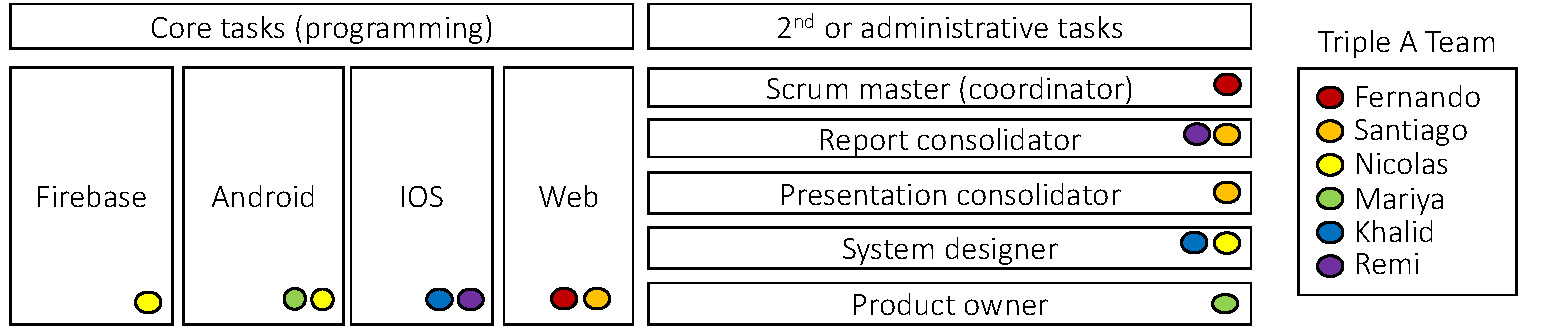
\includegraphics[width=1\textwidth]{figs/tasks}
	\caption{Tasks allocation}
	\label{fig:Tasks}
\end{figure}



5.2. Decision Making and Conflict Resolutions

Making agile agreements and rapidly solve conflicts is a key driver to maximise our team output. Our methodology is inspired in the agents and multiagent theory ~\cite{4646etyet}, specifically in a practical reasoning agent BDI (Belief – Desires - Intentions).

In this manner, each team member always have a valid point of view. Any difference between opinions is a deliberation process (where personal conflict is a conciliation process, which is a special type of deliberation), that would transform a set of options to a set of intentions (this implies that each time there is a deliberation process, the first step is to state a set of options). Then we will plan and assign resources. However, the deliberation process required a balance due to time restrictions (based on our timetable and curve advance). This implies that we must state a mechanism to accelerate the process wherever it is appropriated (deliberation process output is the ideal, but in a practical sense no always we will have time for a full consensus).

So, each time that we can’t achieve a full consensus due to time restrictions, we have specified an agreement protocol that precipitated a final decision where the group will be move forward. For this, we use the [1] Borda Count vote procedure, to try to maximise the preferences of all the group.

Finally, for a personal conflict (such as a communication problem), there will be an arbitration protocol to try to solve it. Basically, the team identify those members that are no involving in the conflict in order that they can mediate. If after a conciliation process there is no any agreement, referees will make the decision (only if there are 2 or more referees). If referees declare itself unavailable to reach a final decision, then we will activate the agreement protocol. The following flowchart summarises our methodology.

\begin{figure}[ht]
\centering
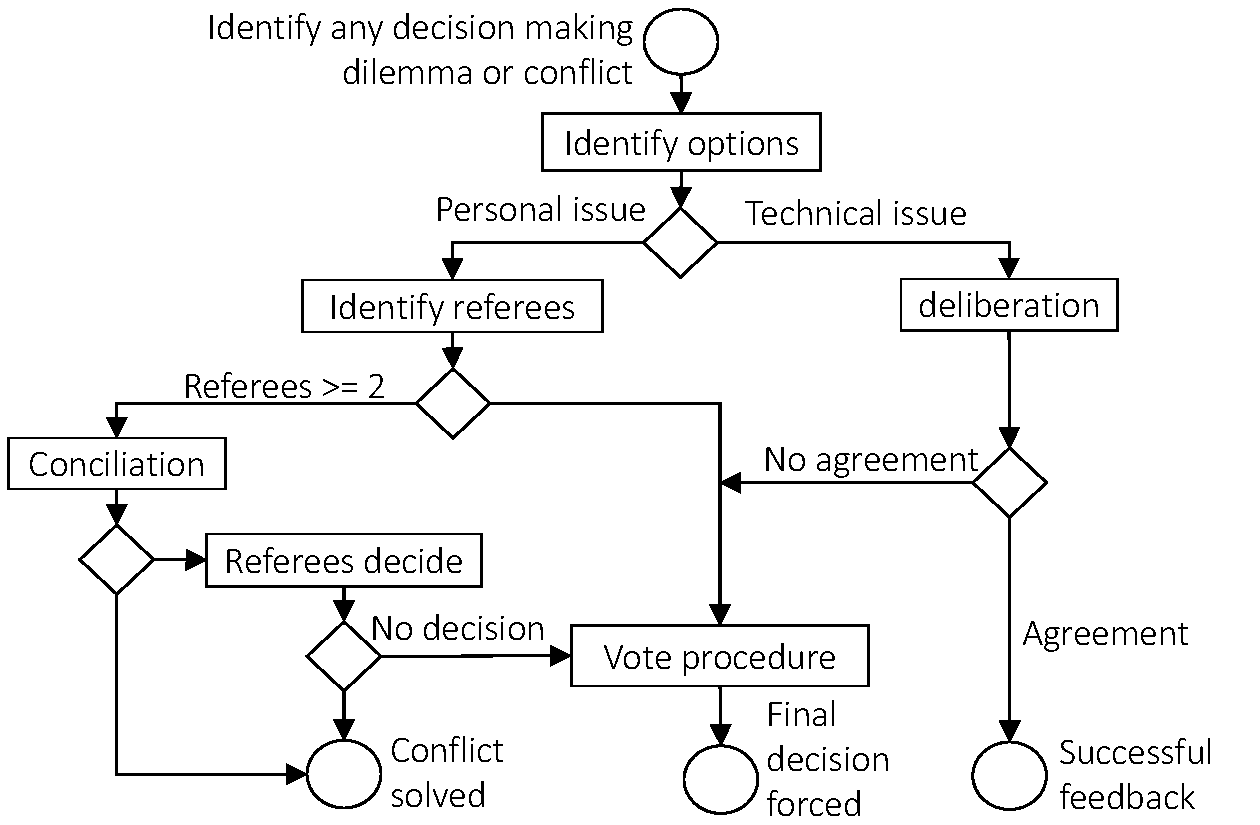
\includegraphics[width=0.6\textwidth]{figs/met}
	\caption{Decision Making and Conflicts Resolution Methodology}
	\label{fig:decisions}
\end{figure}






\subsection{Experiences while working together}

iOS: 
We started by building a simple portal to display grades and scores of students of an institution. It also has the feature of adding a new course and grade. With this simple project, we became more confident on developing iOS chat application, at least up to the level shown on this project. Our application was able to meet the requirements listed under our Priority 1 in Table 1 but for how to search for contacts and use Gmail. We were able to achieve secure connection, messages, contact list, sign in by email, one to one conversation across the platforms.
For the iOS client development, we started with zero experience in Swift and Xcode. 

We are professional of multiple areas and this is a new challenge for us…  (to correct this, but more or less this is the idea…). 
Thus, Agile Methodology requires to be successful in dividing the project in small parts, so each part can be tested while the advance. However, because we don't have an initial detailed division, the advantages of this methodology over the traditional V-model don't apply.  It is true that invest a major portion in planning is better to reduce the time, resources and mistakes in the implementation. However, because we needed to learn and develop some skills while implemented, an ideal plan with proper small division was not achieved. 


